\documentclass[11pt]{beamer}

\graphicspath{{Images/}{./}}
\usepackage{booktabs}
\usetheme{Madrid}

\usefonttheme{default} % Typeset using the default sans serif font

\usepackage{palatino} % Use the Palatino font for serif text

\usepackage[default]{opensans} % Use the Open Sans font for sans serif text

\useinnertheme{circles}

\newcommand{\light}[1]{\textcolor{gray}{#1}}
\usepackage{xcolor}

\title[DSA Scale Uncertainty]{Addressing Scale Uncertainty in Gene and Microbe Set Enrichment Analysis}

\author[Kyle McGovern]{Kyle McGovern}

\institute[Penn State]{The Pennsylvania State University \\ \smallskip \textit{kvm6065@psu.edu}} 

\date[\today]{GLBIO 2024 \\ \today}

%----------------------------------------------------------------------------------------

\begin{document}

%----------------------------------------------------------------------------------------
%	TITLE SLIDE
%----------------------------------------------------------------------------------------

\begin{frame}
	\titlepage % Output the title slide, automatically created using the text entered in the PRESENTATION INFORMATION block above
\end{frame}

\begin{frame}
    \frametitle{Review of Key Concepts}

    Consider an 16S rRNA-seq experiment measuring \(D\) taxa in the colons of \(N\) patients:
    \begin{align*}
      \underbrace{W_{dn}}_{\substack{\text{Absolute Abundance} \\ \text{Taxa d, Patient n} \\ \text{\textcolor{red}{(Unmeasured)}}}} = \underbrace{W^\parallel_{dn}}_{\substack{\text{Composition} \\ \text{Taxa d, Patient n} \\ \text{\textcolor{green}{(Measured)}}}} \times \underbrace{W^\perp_n}_{\substack{\text{Scale} \\ \text{(e.g., total \# of microbes in} \\ \text{patient n's colon)} \\ \text{\textcolor{red}{(Unmeasured)}}}}
    \end{align*}

    \pause

    Consider estimation of the (Log Fold Change) LFC of taxa \(d\) in patients with and without Ulcerative Colitis:
    \begin{align*}
        \underbrace{\theta_d}_{\text{LFC in Absolute Abundance}} &= \underbrace{\theta^{\parallel}_d}_{\text{LFC in Composition}}+\underbrace{\theta^\perp}_{\text{LFC in Scale}}. \nonumber
    \end{align*}

\end{frame}

\begin{frame}
  \frametitle{Review of Key Concepts}

    Methods like ALDEx2, DESeq2, Limma, etc. estimate LFCs using sequence count data \(Y\):
    \begin{align*}
    f(Y) &= \hat{\theta}_d \\
    &= \underbrace{\hat{\theta}^\parallel_d}_{\substack{\text{Estimated LFC in the} \\ \text{\textcolor{green}{measured} composition}}} + \underbrace{\hat{\theta}^\perp}_{\substack{\text{Estimated LFC in the} \\ \text{\textcolor{red}{unmeasured} scale}}}.
    \end{align*}

    \pause

    Estimate \(\hat{\theta}^\perp\) comes from normalization.
    For Example:
    \begin{itemize}
      \item Total Sum Scaling (TSS): \(\hat{\theta}^\perp=0\)
      \pause
      \item Centered Log Ratio (CLR): \(\hat{\theta}^\perp=-\text{mean}(\hat{\theta}^\parallel)\)
    \end{itemize}
\end{frame}

\begin{frame}
  \frametitle{Differential Set Analysis (DSA)}

   This presentation will focus on Differential Set Analysis (DSA) rather than Differential Expression/Abundance (DE/DA)
   \begin{columns}[c]
     \begin{column}{0.5\textwidth}
        \end{column}
        \hspace{-50pt}
        \vrule{}
        \begin{column}{0.50\textwidth}
        \end{column}
   \end{columns}
   
   \begin{block}{Goals of This Presentation}
     \begin{enumerate}
       \item Show that \textbf{\textcolor{red}{incorrect} scale estimates} (i.e., \(\hat{\theta}^\perp\) or \(\hat{W}^\perp\)) inflate false positives in DSA
      \item Propose methods to address these false positives  
     \end{enumerate}
   \end{block}

\end{frame}

\begin{frame}
  \frametitle{GSEA with Gene Label Permutations}

  The GSEA Algorithm Step-by-Step
  \begin{enumerate}
    \item Pick a set of genes \(S\) (e.g., the apoptosis signaling pathway)
    \item Estimate LFCs \(\hat{\theta}=f(Y)\) (i.e., with DESeq2, ALDEx2, limma)
    \item Order the LFCs from largest to smallest
    \begin{figure}
      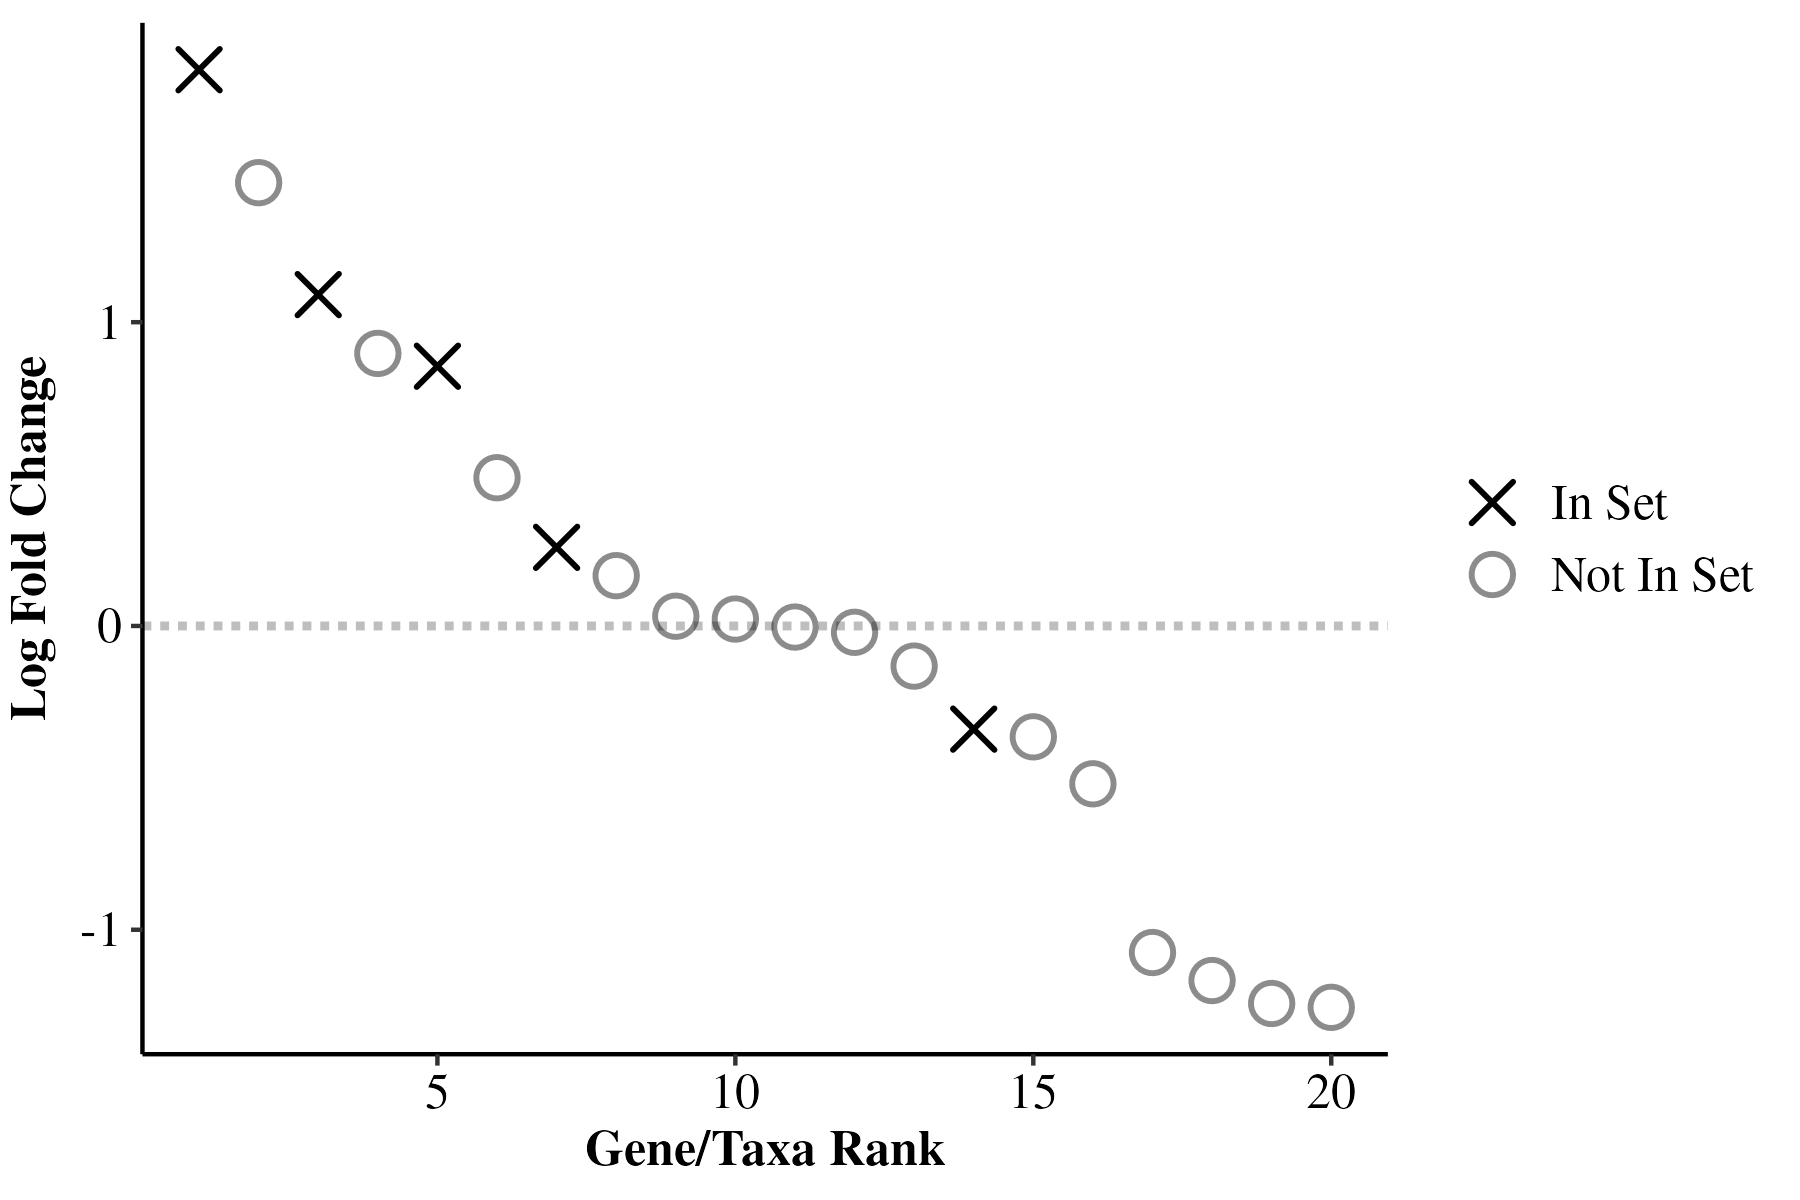
\includegraphics[scale=0.6]{/home/hh/data/output/lfcs_1.png}
      \centering
    \end{figure}
  \end{enumerate}
\end{frame}

\begin{frame}
   \frametitle{GSEA with Gene Label Permutations}

  The GSEA Algorithm Step-by-Step
  \begin{enumerate}
    \setcounter{enumi}{2}
    \item Calculate a running sum \textbf{weighted} by the LFC
    \item Calculate an enrichment score (max distance from \(0\) of \textbf{weighted} running sum)
    \begin{columns}
        \begin{column}{0.5\textwidth}
        \begin{center}
            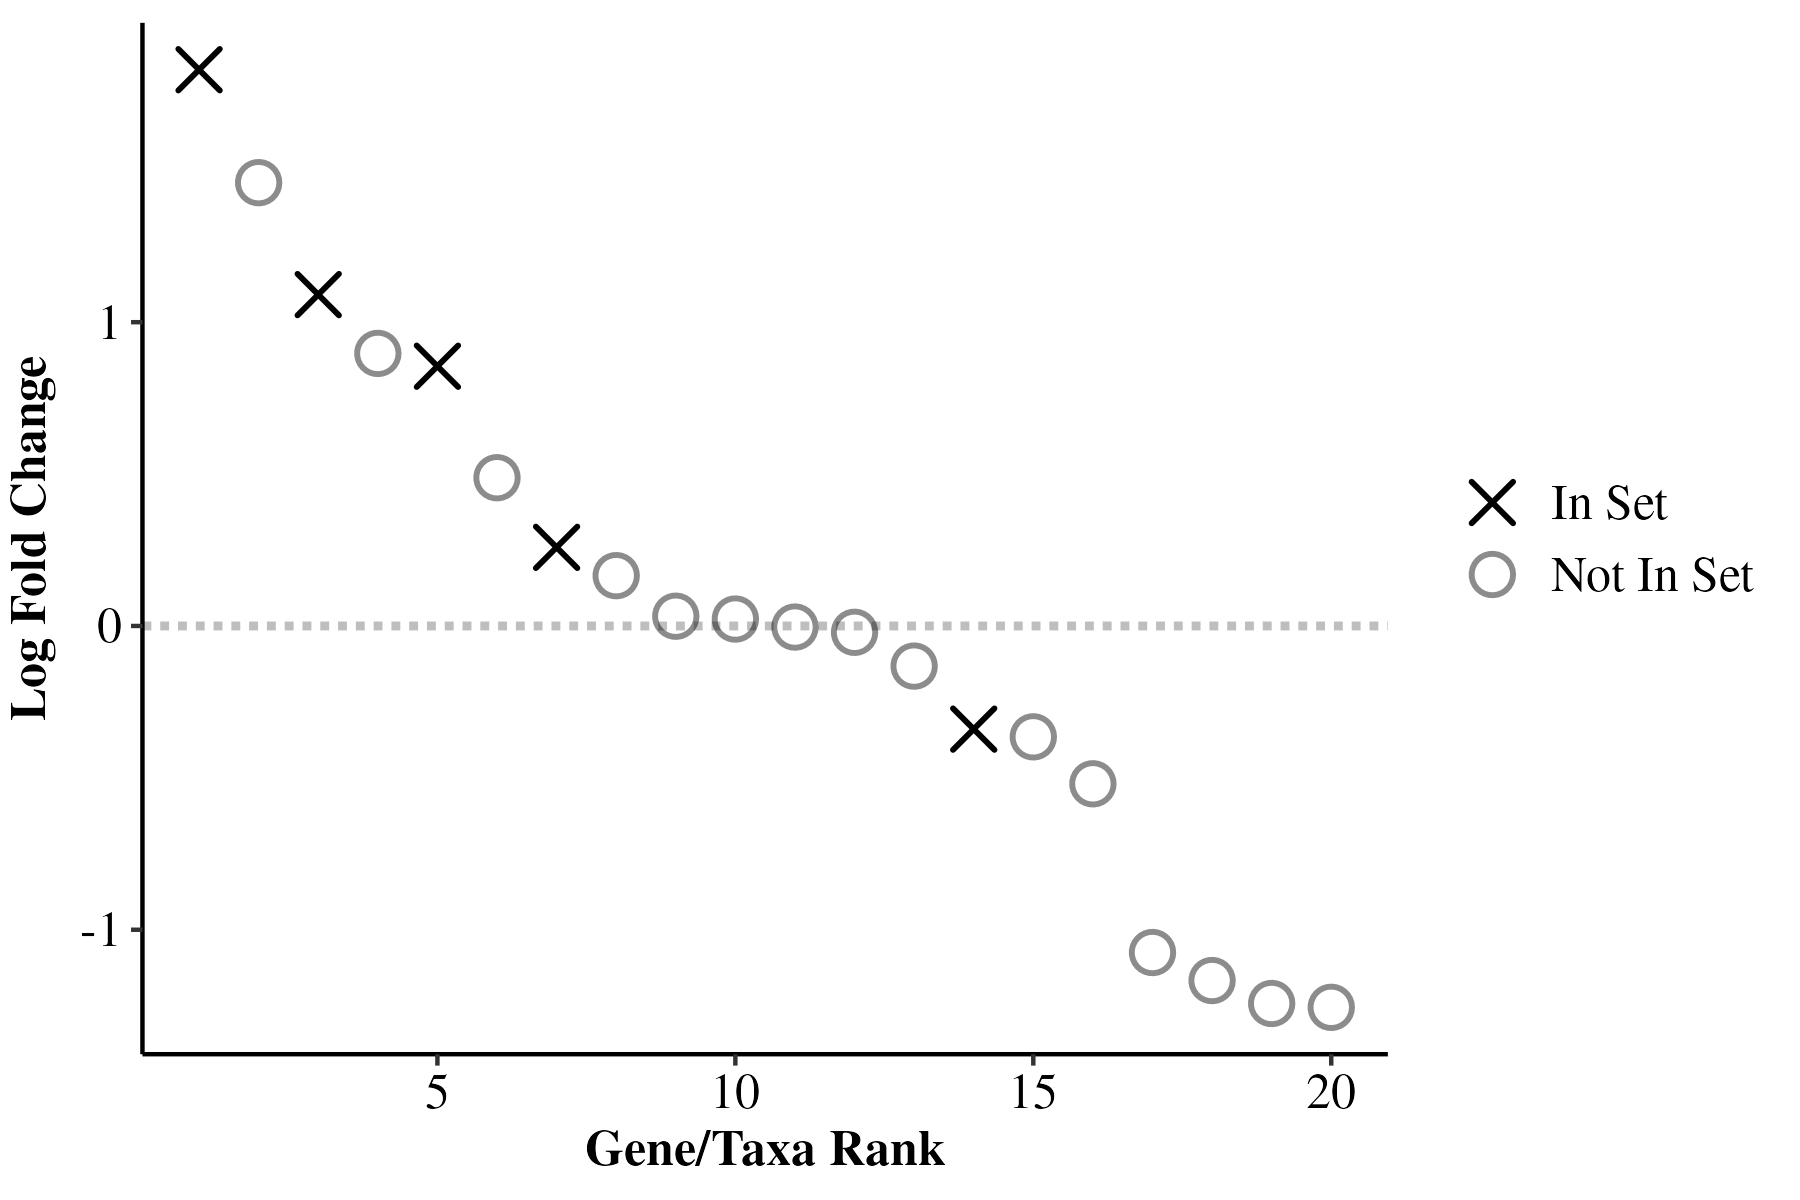
\includegraphics[scale=0.4]{/home/hh/data/output/lfcs_1.png}
        \end{center}
        \end{column}
        \begin{column}{0.5\textwidth}  %%<--- here
        \begin{center}
        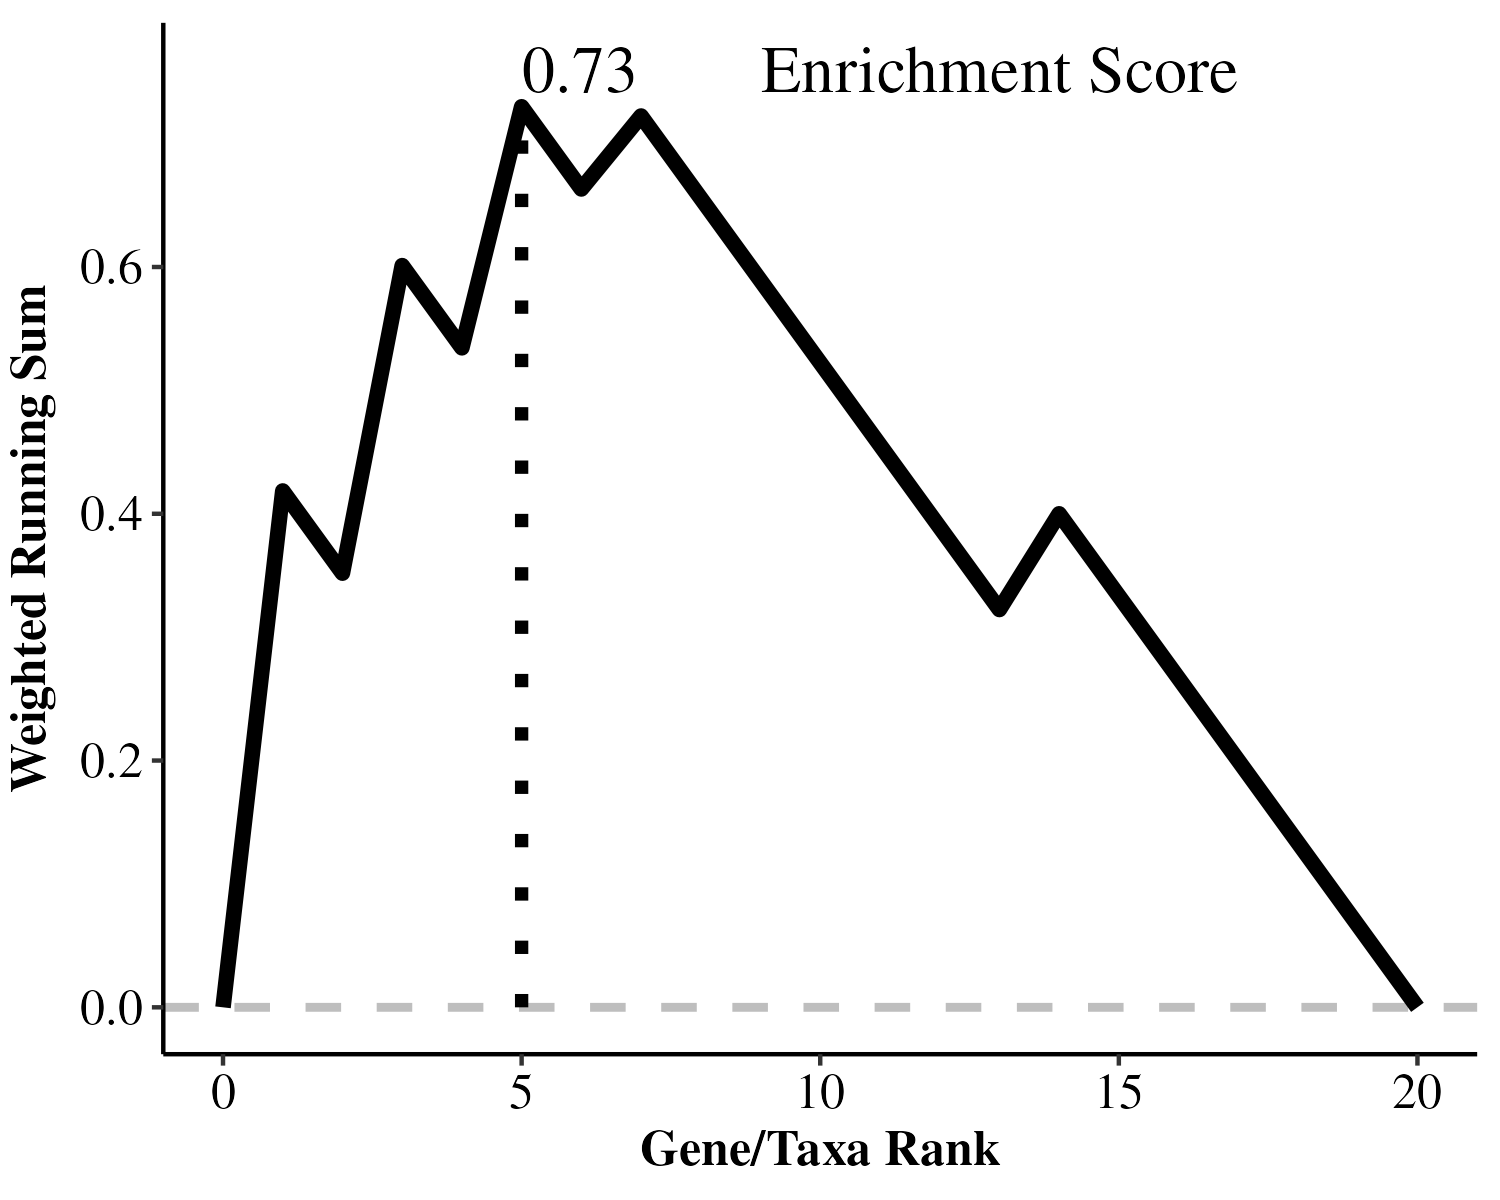
\includegraphics[scale=0.47]{/home/hh/data/output/lfcs_2.png}
        \end{center}
        \end{column}
    \end{columns}
  \end{enumerate} 
\end{frame}

%\begin{frame}
%  \frametitle{GSEA with Gene Label Permutations}
%
%  [PLACEHOLDER Final p-value, 2 examples for intuition]
%\end{frame}

\begin{frame}
  \frametitle{GSEA Target of Inference}

  We can think of the GSEA algorithm as a function of the LFCs:
  \begin{align*}
    \underbrace{\phi_S}_{\substack{\text{DSA Target} \\ \text{Estimand}}} = u(\underbrace{\theta}_{\substack{\text{True, Unkown} \\ \text{LFCs}}})
  \end{align*}

  DSA Target Estimand:
  \begin{align*}
    \phi_S = \begin{cases}
      1 & \text{Gene Set } S \text{ is significantly enriched} \\
      -1 & \text{Gene Set } S \text{ is significantly depleted} \\
      0 & \text{Gene Set } S \text{ is not significantly changing}.
    \end{cases}
  \end{align*}

\end{frame}

\begin{frame}
  We want to estimate enrichment with the true LFC \(\theta\):
  \begin{align*}
    \phi_S = u(\theta)
  \end{align*}

  \pause

  But we don't know the true LFC \(\theta\)! So instead we estimate:
  \begin{align*}
    \hat{\phi}_S &= u(\hat{\theta}) \\
                 &= u(\hat{\theta}^\parallel+\hat{\theta}^\perp).
  \end{align*}

  \pause
  
  The scale \(\theta^\perp\) is \textcolor{red}{unmeasured}, so what if our estimate \(\hat{\theta}^\perp\) is wrong?
\end{frame}

\begin{frame}
  \frametitle{LFC Sensitivity Analysis}

  Consider error \(\epsilon^\perp\) in our estimate of the unmeasured scale \(\theta^\perp\):
  \begin{align*}
    \underbrace{\theta^\perp}_{\text{True LFC in Scale}} = \underbrace{\hat{\theta}^\perp}_{\text{Estimate}} + \underbrace{\pmb{1}\epsilon^\perp}_{\text{Estimation Error}}
  \end{align*}

  \pause
  
    We can use \(\epsilon^\perp\) to learn how sensitive the \textbf{truth} \(\phi_S\) is to error:
    \begin{align*}
      \phi_s &= u(\hat{\theta}^\parallel+ \hat{\theta}^\perp + \pmb{1}\epsilon^\perp) \\
           &= u(\hat{\theta}+\pmb{1}\epsilon^\perp)
    \end{align*}
  
  \pause

  LFC Sensitivity Analysis Algorithm:
  \begin{enumerate}
      \item Get estimated LFCs \(\hat{\theta}\) (e.g., from ALDEx2, limma, DESeq2, etc.)
      \item Estimate set enrichment/depletion for set \(S\): \(\hat{\phi}_S=u(\hat{\theta})\)
      \item Compare estimate (\(\hat{\phi}_S\)) to truth (\(\phi_S\)) under different amounts of error \(\epsilon^\perp\)
  \end{enumerate}

\end{frame}

\begin{frame}
  \frametitle{Interpreting Error \(\epsilon^\perp\) and LFC Sensitivity Analysis Results}

  Consider error \(\epsilon^\perp = \pm 0.5\):
  \begin{enumerate}
  \item This error corresponds to the true \(\theta^\perp\) being \(e^{0.5}=1.65\) times lower/higher than \(\hat{\theta}^\perp\)
    \pause
    \item Example results if a Gene set \(S\) is sensitive to error:
      \begin{center}
        \begin{tabular}{ |c|c|c| } 
        \hline
        \(\epsilon^\perp=-0.5\) & \(\epsilon^\perp=0\) & \(\epsilon^\perp=0.5\) \\
        \hline
        \(\phi_S=0\) & \(\phi_S=1\) & \(\phi_S=0\) \\
        \hline
        \end{tabular}
      \end{center}
    \pause
    \item Example results if a Gene set \(S\) is not sensitive to error:
      \begin{center}
        \begin{tabular}{ |c|c|c| }
        \hline
        \(\epsilon^\perp=-0.5\) & \(\epsilon^\perp=0\) & \(\epsilon^\perp=0.5\) \\
        \hline
        \(\phi_S=1\) & \(\phi_S=1\) & \(\phi_S=1\) \\
        \hline
        \end{tabular}
      \end{center}
  \end{enumerate}
\end{frame}

\begin{frame}
  \frametitle{LFC Sensitivity Analysis Simulation}
  
  \begin{center}
    \includegraphics[scale=0.65]{/home/hh/data/output/journal.pcbi.1011659.g001.PNG}
  \end{center}

  Note: PPV (Positive Predictive Value) is the \% of positives that are true positives
 
\end{frame}

\begin{frame}
  \frametitle{Multiple Simulations of Different LFC Distributions, Gene Set Sizes, and Total \#'s of Genes}
  \begin{center}
    \includegraphics[scale=0.185]{/home/hh/data/output/fig_mult_sim.png}
  \end{center}
\end{frame}
  
\begin{frame}
  \frametitle{Real Data Analysis}

  Real Data Analysis:
  \begin{enumerate}
    \item RNA-seq: normal-adjacent-to-tumor vs healthy thtroid tissue
    \item LFCs estimated with Songbird (Morton et al., 2019), GSEA performed with fgsea (Korotkevich et al., 2021)
  \end{enumerate}

  \pause

  fgsea results for the Inflammatory Response Pathway:
  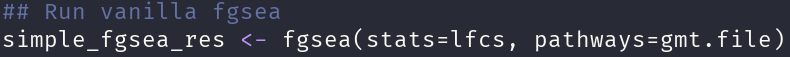
\includegraphics[scale=0.30]{/home/hh/data/output/vanilla_fgsea.png}
    \begin{center}
    \begin{tabular}{ |c|c| }
    \hline
    Enrichment Score & Adjusted p-value \\
    \hline
    \textcolor{blue}{1.53} & \textcolor{red}{0.003}  \\
    \hline
    \end{tabular}
    \end{center}
 
  \pause
  LFC Sensitvity Results:
  \includegraphics[scale=0.30]{/home/hh/data/output/LFCS_fgsea.png}
    \begin{center}
    \begin{tabular}{ |c|c|c| }
    \hline
    \(\epsilon^\perp\) & Enrichment Score & Adjusted p-value \\
    \hline
    -0.5 & \textcolor{red}{-0.89} & 1  \\
    \hline
    0 & \textcolor{blue}{1.53} & \textcolor{red}{0.003}  \\
    \hline
    0.5 & \textcolor{blue}{1.5} & \textcolor{red}{0}  \\
    \hline
    \end{tabular}
    \end{center}

\end{frame}

\begin{frame}
  \frametitle{Complete Results for Real Data Analysis}
  
  \includegraphics[scale=0.75]{/home/hh/data/output/journal.pcbi.1011659.g002.PNG}
\end{frame}

\begin{frame}
  \frametitle{Two Alternatives to LFC Senstivity Analysis}

  To address false positives in GSEA I present two additional methods:
  \pause
  \begin{enumerate}
  \item \underline{The LFC Sensitivity Test}

    \vspace{5px}
    Let \(p_{\epsilon^\perp}\) be the GSEA p-value at \(\epsilon^\perp\). The LFC Sensitivity Test's new p-value:
    \begin{align*}
      p=\sup_{\epsilon^\perp \in (-\infty, \infty)} p_{\epsilon^\perp}
    \end{align*}

    This test has non-zero power in real data analysis:
    \begin{center}
      \includegraphics[scale=0.12]{/home/hh/data/output/power.png}
    \end{center}


  \end{enumerate}  
\end{frame}

\begin{frame}
  \frametitle{Two Alternatives to LFC Senstivity Analysis}
  To address false positives in GSEA I present two additional methods:
  \begin{enumerate}
   \setcounter{enumi}{1}
   \item \underline{GSEA with Compositional Weighting (GSEA-CW)}

    \vspace{5px}
    The GSEA target estimand (i.e., goal of inference) is
    \begin{align*}
      \phi_S = u(\theta)
    \end{align*}

    A different target estimand (using the CLR) implies a different inferential goal:
    \begin{align*}
      \psi_S &= u(\theta-\text{mean}(\theta)) \\
      &= u(\theta^\parallel+\theta^\perp-\text{mean}(\theta^\parallel)-\theta^\perp) \\
      &= u(\theta^\parallel-\text{mean}(\theta^\parallel))
    \end{align*}
    
  \end{enumerate}
\end{frame}
  
\begin{frame}
  \frametitle{DSA Methods that Account for Inter-gene/inter-entity Correlations}
  Inter-gene/taxa correlations can massively inflate the false positive rate of GSEA with gene label permutations (Gatti et al., 2010)

  \begin{center}
    \includegraphics[scale=0.12]{/home/hh/data/output/correlations.png}
  \end{center}
  
  Two methods that handle inter-gene/taxa correlations:
  \begin{enumerate}
    \item GSEA with \textbf{sample label} permutations
    \item limma's CAMERA method
  \end{enumerate}
  
\end{frame}

\begin{frame}
  \frametitle{The CAMERA Method}
  

  Two methods that handle inter-gene/taxa correlations:
  \begin{enumerate}
  \item GSEA with \textbf{sample label} permutations
   \vspace{10px}
    
   Rather than permute gene set \(S\); estimate absolute abundances \(\hat{W}\), permute sample labels, and re-estimate the LFC \(\hat{\theta}\).

   \pause
    
  \item limma's CAMERA method

    \vspace{10px}
    A two-sample t-test for the set \(S\) that uses a Variance Inflation Factor (VIF) to account for correlation:
    \begin{align*}
      \frac{\hat{\theta}_{\in S} - \hat{\theta}_{\notin S}}{s_p\sqrt{\text{VIF}/m_1+1/m_0}}
    \end{align*} 

  \end{enumerate}
\end{frame}

\begin{frame}
  \frametitle{Scale Sensitivity Analyses}
   \begin{center}
    \includegraphics[scale=0.18]{/home/hh/data/output/camera.png}
   \end{center}

   \footnotesize{* GSEA-LFC-S is GSEA with sample label permutations, GSEA-CW-S is GSEA with compositional weighting and sample label permutations}
\end{frame}

\begin{frame}
  \frametitle{Future Directions}
  In the LFC Sensitivity Test we calculate a p-value:
  \begin{align*}
    p= \sup_{\epsilon^\perp \in (-\infty, \infty)} p_{\epsilon^\perp}.
  \end{align*}
  But why consider all possible scale assumptions?

  \pause
  \vspace{10px}
  For instance \(\theta^\perp=10\) implies a \(e^{10}=22026\) fold increase in scale!

  \pause
  \vspace{10px}
  Consider a reseacher willing to make an \textit{interval assumption} \(\epsilon^\perp \in [-1,1]\):
  \begin{align*}
    p= \sup_{\epsilon^\perp \in [-1, 1]} p_{\epsilon^\perp}.
  \end{align*}
  This could be useful beyond GSEA, but \textbf{differential expression/abundance as well(!)}
 
\end{frame}

\end{document} 
